% Created 2023-06-25 Sun 23:50
% Intended LaTeX compiler: lualatex
\documentclass[bigger]{beamer}
\usepackage{graphicx}
\usepackage{longtable}
\usepackage{wrapfig}
\usepackage{rotating}
\usepackage[normalem]{ulem}
\usepackage{amsmath}
\usepackage{amssymb}
\usepackage{capt-of}
\usepackage{hyperref}
\usetheme[progressbar=foot, sectionpage=none, numbering=fraction]{metropolis}
\usepackage{tikz}
\usetikzlibrary{automata, positioning, arrows, arrows.meta}
\tikzstyle{mynode}=[thick,draw=blue,fill=blue!20,circle,minimum size=22]
\usepackage{booktabs}
\usepackage{adjustbox}
\usepackage{diagbox}
\usepackage{latexcolors}
\usepackage{diagbox}
\usepackage{dsfont}
\usepackage{amsmath}
\usepackage{fontawesome5}
\usepackage{listofitems}
\usepackage[ruled]{algorithm2e}
\definecolor{RedBrown}{RGB}{192, 4, 4} \setbeamercolor{progress bar}{fg=RedBrown} \setbeamercolor{title separator}{fg=RedBrown}
\setbeamercolor{progress bar in head/foot}{fg=RedBrown} \setbeamercolor{progress bar in section page}{fg=RedBrown} \setbeamercolor{alerted text}{fg=RedBrown}
\pretocmd{\tableofcontents}{\thispagestyle{empty}}{}{}
\addtocounter{framenumber}{-1}
\usepackage{listings}
\usepackage{xcolor}
\definecolor{codegreen}{rgb}{0,0.6,0}
\definecolor{codegray}{rgb}{0.5,0.5,0.5}
\definecolor{codepurple}{rgb}{0.58,0,0.82}
\definecolor{backcolour}{HTML}{f0f0f0}
\lstdefinestyle{mystyle}{
backgroundcolor=\color{backcolour},
commentstyle=\color{codegreen},
keywordstyle=\color{magenta},
numberstyle=\tiny\color{codegray},
stringstyle=\color{codepurple},
basicstyle=\ttfamily,
breakatwhitespace=false,
breaklines=true,
captionpos=b,
keepspaces=true,
numbers=none,
numbersep=5pt,
showspaces=false,
showstringspaces=false,
showtabs=false,
tabsize=2
}
\lstset{style=mystyle}
\usepackage[outline]{contour} % glow around text
\contourlength{1.4pt}
\tikzset{>=latex} % for LaTeX arrow head
\usepackage{xcolor}
\colorlet{myred}{red!80!black}
\colorlet{myblue}{blue!80!black}
\colorlet{mygreen}{green!60!black}
\colorlet{myorange}{orange!70!red!60!black}
\colorlet{mydarkred}{red!30!black}
\colorlet{mydarkblue}{blue!40!black}
\colorlet{mydarkgreen}{green!30!black}
\tikzstyle{node}=[thick,circle,draw=myblue,minimum size=22,inner sep=0.5,outer sep=0.6]
\tikzstyle{node in}=[node,green!20!black,draw=mygreen!30!black,fill=mygreen!25]
\tikzstyle{node hidden}=[node,blue!20!black,draw=myblue!30!black,fill=myblue!20]
\tikzstyle{node convol}=[node,orange!20!black,draw=myorange!30!black,fill=myorange!20]
\tikzstyle{node out}=[node,red!20!black,draw=myred!30!black,fill=myred!20]
\tikzstyle{connect}=[thick,mydarkblue] %,line cap=round
\tikzstyle{connect arrow}=[-{Latex[length=4,width=3.5]},thick,mydarkblue,shorten <=0.5,shorten >=1]
\tikzset{ % node styles, numbered for easy mapping with \nstyle
node 1/.style={node in},
node 2/.style={node hidden},
node 3/.style={node out},
}
\def\nstyle{int(\lay<\Nnodlen?min(2,\lay):3)} % map layer number onto 1, 2, or 3
\usetheme{default}
\author{Andrea Pierré}
\date{June 26, 2023}
\title{Joint RL meeting}
\institute{Brown University}
\titlegraphic{\hfill\includegraphics[height=1.5cm]{img/Brown Logo_2016_2 Color Process ST_1300.png}}
\setbeamercovered{transparent=10}
\setbeamertemplate{section in toc}[sections numbered]
\AtBeginSection[]{\begin{frame}[plain, noframenumbering]{Outline}    \setbeamertemplate{section in toc}[sections numbered]\setbeamertemplate{subsection in toc}[subsections numbered]\tableofcontents[currentsection, currentsubsection]\end{frame}}
\AtBeginSubsection[]{\begin{frame}[plain, noframenumbering]{Outline}\setbeamertemplate{section in toc}[sections numbered]\setbeamertemplate{subsection in toc}[subsections numbered]\tableofcontents[currentsection,currentsubsection]\end{frame}}
\hypersetup{
 pdfauthor={Andrea Pierré},
 pdftitle={Joint RL meeting},
 pdfkeywords={},
 pdfsubject={},
 pdfcreator={Emacs 28.2 (Org mode 9.6)}, 
 pdflang={English}}
\begin{document}

\maketitle
\begin{frame}[plain]{Outline}
\tableofcontents
\end{frame}

\section{Reducing the number of features in function approximation}
\label{sec:org1f3d9c9}
\begin{frame}[label={sec:orgf84cdaf}]{Features matrix -- allocentric agent}
\(\to\) Reduced from 100 to 25 locations + 4 cues
\begin{center}
\includegraphics[height=0.8\textheight]{img/FuncApprox-allo-features-matrix.png}
\end{center}
\end{frame}
\begin{frame}[label={sec:org9d007fb}]{Rewards and steps -- allocentric agent}
\begin{center}
\includegraphics[width=\textwidth]{img/FuncApprox-allo-rewards-steps.png}
\end{center}
\end{frame}
\begin{frame}[label={sec:org6f1c2b2}]{Q-values learned -- allocentric agent}
\begin{center}
\includegraphics[width=.9\linewidth]{img/FuncApprox-allo-q-values.png}
\end{center}
\end{frame}
\begin{frame}[label={sec:org14c38a0}]{Features matrix -- egocentric agent}
\(\to\) Reduced from 400 to 100 locations (25 locations x 4 head directions) + 16 cues (4 cues x 4 head directions)
\begin{center}
\includegraphics[height=0.75\textheight]{img/FuncApprox-ego-features-matrix.png}
\end{center}
\end{frame}
\begin{frame}[label={sec:org6735624}]{Rewards and steps -- egocentric agent}
\begin{center}
\includegraphics[width=\textwidth]{img/FuncApprox-ego-rewards-steps.png}
\end{center}
\end{frame}
\begin{frame}[label={sec:org353ea85}]{Q-values learned -- egocentric agent}
\begin{center}
\includegraphics[width=.9\linewidth]{img/FuncApprox-ego-q-values.png}
\end{center}
\end{frame}
\section{Deep RL -- first draft \& issues}
\label{sec:orgc833944}
\begin{frame}[label={sec:org1881447}]{Toy task : Random Walk 1D}
\begin{center}
\includegraphics[width=.9\linewidth]{img/RandomWalk1D-transparent.png}
\end{center}
\end{frame}
\begin{frame}[label={sec:orgb8dd11b}]{Network used}
% https://tikz.net/neural_networks/
\begin{center}
\begin{adjustbox}{max height=\textheight, keepaspectratio}
% NEURAL NETWORK no text
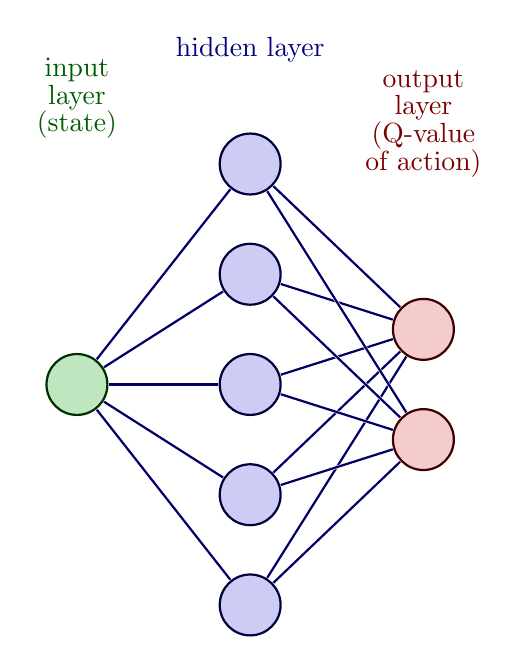
\begin{tikzpicture}[x=2.2cm,y=1.4cm]
  \message{^^JNeural network without text}
  \readlist\Nnod{1,5,2} % array of number of nodes per layer

  \message{^^J  Layer}
  \foreachitem \N \in \Nnod{ % loop over layers
    \def\lay{\Ncnt} % alias of index of current layer
    \pgfmathsetmacro\prev{int(\Ncnt-1)} % number of previous layer
    \message{\lay,}
    \foreach \i [evaluate={\y=\N/2-\i; \x=\lay; \n=\nstyle;}] in {1,...,\N}{ % loop over nodes

      % NODES
      \node[node \n] (N\lay-\i) at (\x,\y) {};

      % CONNECTIONS
      \ifnum\lay>1 % connect to previous layer
        \foreach \j in {1,...,\Nnod[\prev]}{ % loop over nodes in previous layer
          \draw[connect,white,line width=1.2] (N\prev-\j) -- (N\lay-\i);
          \draw[connect] (N\prev-\j) -- (N\lay-\i);
          %\draw[connect] (N\prev-\j.0) -- (N\lay-\i.180); % connect to left
        }
      \fi % else: nothing to connect first layer

    }
  }

  % LABELS
  \node[above=1.85,align=center,mygreen!60!black] at (N1-1.90) {input\\[-0.2em]layer\\[-0.2em](state)};
  \node[above=0.55,align=center,myblue!60!black] at (N2-1.90) {hidden layer};
  \node[above=1,align=center,myred!60!black] at (N\Nnodlen-1.90) {output\\[-0.2em]layer\\[-0.2em](Q-value\\[-0.2em]of action)};

\end{tikzpicture}
\end{adjustbox}
\end{center}
\end{frame}
\begin{frame}[label={sec:org94344ed}]{States and actions}
\begin{center}
\includegraphics[width=.9\linewidth]{img/DRL-states-actions.png}
\end{center}
\begin{center}
\includegraphics[width=.9\linewidth]{img/DRL-states-actions2.png}
\end{center}
\end{frame}
\begin{frame}[label={sec:org10dfb92}]{Rewards and steps}
\begin{center}
\includegraphics[width=.9\linewidth]{img/DRL-rewards-steps.png}
\end{center}
\begin{center}
\includegraphics[width=.9\linewidth]{img/DRL-rewards-steps2.png}
\end{center}
\end{frame}
\begin{frame}[label={sec:orgd88bf50}]{Q-values learned}
\begin{center}
\includegraphics[width=\textwidth]{img/DRL-q-values.png}
\end{center}
\begin{center}
\includegraphics[width=\textwidth]{img/DRL-q-values2.png}
\end{center}
\end{frame}
\begin{frame}[label={sec:org8f4cbeb}]{Network loss}
\begin{columns}
\begin{column}{0.5\columnwidth}
\centering
Right leaning
\begin{center}
\includegraphics[width=\columnwidth]{img/DRL-loss.png}
\end{center}
\end{column}
\begin{column}{0.5\columnwidth}
\centering
Left leaning
\begin{center}
\includegraphics[width=\columnwidth]{img/DRL-loss2.png}
\end{center}
\end{column}
\end{columns}
\end{frame}
\begin{frame}[label={sec:orge74e4b4}]{Network weights}
\centering
\scriptsize
Right leaning
\vspace{-1em}
\begin{center}
\includegraphics[width=\textwidth]{img/DRL-weights.png}
\end{center}

\vspace{-1em}
\centering
\scriptsize
Left leaning
\vspace{-1em}
\begin{center}
\includegraphics[width=\textwidth]{img/DRL-weights2.png}
\end{center}
\end{frame}
\begin{frame}[label={sec:org163efb6}]{Network gradients}
\centering
\scriptsize
Right leaning
\vspace{-1em}
\begin{center}
\includegraphics[width=\textwidth]{img/DRL-gradients.png}
\end{center}

\vspace{-1em}
\centering
\scriptsize
Left leaning
\vspace{-1em}
\begin{center}
\includegraphics[width=\textwidth]{img/DRL-gradients2.png}
\end{center}
\end{frame}
\begin{frame}[label={sec:org865fe73},standout]{~}
Questions ?
\end{frame}
\end{document}
